\documentclass[11pt]{article}
\usepackage{mypackages}
\begin{document}

\maketitle

\section{Introduction}

The natural way of learning is through repeatedly solving the same
task over and over again, each time observing the result and connecting
actions with outcomes.
In the context of machine learning these principles are used
to find the actions that provide the best outcome - a technique known as
\textit{Reinforcement learning}.

The goal of this project is to investigate the advantages of asynchronous reinforcement
learning in an advanced setting - learning to play Atari 2600 games\cite{openAIEnvs}.

Solving a task consists of being in a certain state and making a decision 
which then leads
to a new state, with a new set of decisions to be made, until
a terminal state is reached.
The terminal state is reached when there are no more decisions to be made
and the task is solved.
This means that a task can be seen as a \textit{decision tree}, with actions connecting states to future states.
%%%%%% Task decision tree
\begin{figure}[H]
    \centering
    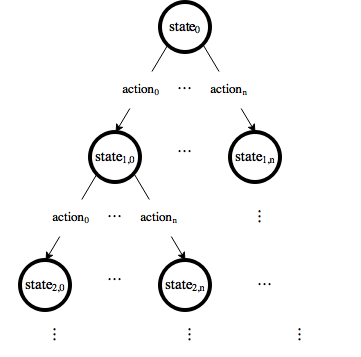
\includegraphics[scale=0.5]{include/decision_tree.png}
    \caption{A decision tree for solving a task.}
    \label{fig:dec_tree}
\end{figure}

In a typical reinforcement learning setting a problem is solved
by moving through the decision tree until a terminal state is reached.
The total result or reward of taking this exact path is then
taken into account the next time the algorithm tries to solve the problem.
The advantage of asynchronous learning is that multiple different paths
can be explored simultanously, which means that learning can happen at
a higher pace.

\subsection{Inspiration}

In december 2013 the DeepMind Technologies team published an article
about an approach to learning from a high dimensional sensory input
using deep reinforcement learning\cite{dqn}.
With a combination of convolutional nerual networks (CNN) and
the reinforcement learning method Q-learning\cite{RLbook}, they
presented results proving that it was possible to learn to play Atari
2600 games at a superhuman level.

Previously reinforcement learning haven't been able to learn to play
advanced games, except for backgammon\cite{tdgammon},
but the combination of deep learning and reinforcement learning
have made it possible.



An example of asynchronous reinforcement learning was presented by the
Google DeepMind team collaborating with the Montreal Institue for Learning
Algorithms (MILA) in an article from june 2016, where multiple different
reinforcement learning algorithms were implemented to take advantage of
asynchronous learning\cite{a3c}.

One of the  algorithms that were implemented asynchronously
was \textit{advantage actor-critic} (A3C), which we will use in this
project to play Atari 2600 games.


%\printbibliography
%\bibliography{citations}
%\bibliographystyle{plain}
\end{document}
